\RequirePackage{ifpdf}
\documentclass[letterpaper,landscape]{slides}
%\documentclass[letterpaper,portrait]{slides}
\usepackage{boxedminipage}

%\input /u/rhl/TeX/pdf.tex
\input pdf.tex

\newif\ifTalk\Talktrue		% We generating a talk, not printing
%\Talkfalse			% no; we're really printing

%\pagestyle{empty}
\setlength{\topmargin}{-1in}
\setlength{\textheight}{7.5in}
\setlength{\textwidth}{9in}
\setlength{\oddsidemargin}{0pt}
\setlength{\oddsidemargin}{0pt}

%\onlyslides{1-3,4,10-9999}
%\onlyslides{26-9999}

\begin{document}

\newcommand{\XXX}[1]{\textbf{XXX} #1}
\newcommand{\colour}[1]{\color{#1}}

\def\eq#1{\begin{equation} \color{blue} #1 \end{equation}}
\def\vx{{\bf x}}
\def\vv{{\bf v}}
\def\p{\partial}
\def\b#1{{\bf  #1}}
\def\p{\partial}
\def\th{^{th}}
\def\msun{{\rm\,M_\odot}}
\def\bnabla{{\bf\nabla}}
\def\dint{\int\!\!\!\int}
\def\d{{\rm d}}
\def\i{{\rm i}}
\def\ddt#1{{\rm{d} #1\over {\rm dt}}}
\def\ddtS#1{{\rm{d^2} #1\over {\rm dt^2}}}
%\lta and \gta produce > and < signs with twiddle underneath
\def\spose#1{\hbox to 0pt{#1\hss}}
\def\lta{\mathrel{\spose{\lower 3pt\hbox{$\mathchar"218$}}
     \raise 2.0pt\hbox{$\mathchar"13C$}}}
\def\gta{\mathrel{\spose{\lower 3pt\hbox{$\mathchar"218$}}
     \raise 2.0pt\hbox{$\mathchar"13E$}}}
\def\mspace{\hbox{\quad}}
\def\deffn#1{{\bf#1}}\def\eqs#1{equations \rf#1}






\newcount\itemCnt\itemCnt=0
\newcommand{\nitem}{%
  \global\advance\itemCnt by 1
  ~\vskip0cm\the\itemCnt.\qquad}

\definecolor{orange}{rgb}{1.0, 0.5, 0.0}
\definecolor{purple}{cmyk}{0.4, 0.8, 0.3, 0.0}


%%%%%%%%%%%%%%%%%%%%%%%%%%%%%%%%%%%
\newcommand{\onepic}[6]{%
\begin{slide}
     \begin{center}
        \begin{minipage}{#1in}
            {\large \color{blue} #6}
            \phantom{x} \vskip #2in
            \phantom{x} \hskip #3in
            {\scalebox{#4}{\includegraphics{#5}}}   
        \end{minipage}
     \end{center}
    \vfill
\end{slide}
}


%%%%%%%%%%%%%%%%%%%%%%%%%%%%%%%%%%%
\newcommand{\picslide}[7]{%
  \begin{slide}
     \begin{center}
        \begin{minipage}{#5in}
            \hskip #6in
            \hskip -1in
            {\scalebox{#4}{\includegraphics{#1.#2}}}
            \vskip #7in~
            {\large \color{blue} #3}
        \end{minipage}
     \end{center}
     \vfill
  \end{slide}
}
%%%%%%%%%%%%%%%%%%%%%%%%%%%%%%%%%%%
 

%%%%%%%%%%%%%%%%%%%%%%%%%%%%%%%%%%%
\newcommand{\Spicslide}[7]{%
  \begin{slide}
     \begin{center}
        \begin{minipage}{#5in}
            \vskip #6in
            \hskip #7in
            {\scalebox{#4}{\includegraphics{#1.#2}}}
        \end{minipage}
     \end{center}
     \vfill
  \end{slide}
}
%%%%%%%%%%%%%%%%%%%%%%%%%%%%%%%%%%%
 



%------------------------------------------------------------------------------

\begin{slide}

\phantom{x}
\vskip -2in
\begin{center}
\bfseries
{\large {\color{blue} Astr 511: Galaxies as galaxies}}
\end{center}

{\centerline {{\color{blue} 
Winter Quarter 2017, University of Washington}}}
{\centerline {{\color{blue} 
Mario Juri\'{c} \& \v{Z}eljko Ivezi\'{c} }}}

\vskip 1.6in

{\centerline {\Large {\color{red}      Lecture 6:             }}}
\vskip 0.2in 
{\centerline {\huge {\color{blue} Dynamics I: Potentials and Orbits }}}

\vfill
\end{slide}
%------------------------------------------------------------------------------

%------------------------------------------------------------------------------
\begin{slide}
\begin{center}
{\large \color{red} 
          Motivation: Understanding the Structure of Galaxies }
\end{center}

Over the past few weeks we've discussed the phenomenology of galaxies: their
shapes, sizes, luminosities, and luminosity profiles, their kinematics 
(velocities of their constituent stars and gas).

We've seen that there are {\em empirical relationships} between many of
these properties (e.g., the Faber-Jackson relation and the fundamental plane,
the Tully Fisher relation, $M - \sigma$ relation, etc.).

These connections are not surprising: many of them are a manifestation of
the underlying {\em dynamics} of the system. In a series of lectures to
follow we will look at using dynamics to understand the observational
relationships, but {\em \bf also tease out otherwise hidden implications}
and insight on the internal structure of galaxies from the observational data.

\vfill
\end{slide}


%------------------------------------------------------------------------------

%------------------------------------------------------------------------------
\begin{slide}
\begin{center}
\bfseries
{\large {\color{blue} Outline} }
\end{center}
\vskip -0.3in

\begin{enumerate}
   \item {\bf \color{blue} Introduction to potentials and orbits}
     \begin{itemize}
             \item {\bf Spherical potentials}
             \item {\bf Axial potentials}
             \item {\bf Stellar orbits}
             \item {\bf Epicycle approximation}
     \end{itemize}
\end{enumerate}

{\color{red} \bf Reading:}
\begin{itemize}
   \item {\color{blue} Binney \& Merrifield:} ch. 10
   \item {\color{blue} Binney \& Tremaine:} chs. 2 \& 3
\end{itemize}

\vfill
\end{slide}
 
%------------------------------------------------------------------------------

%------------------------------------------------------------------------------
\begin{slide}
\begin{center}
\bfseries
{\large {\color{blue} Matter distribution, potentials, orbits ...} }
\end{center}
\vskip -0.3in

\begin{enumerate}
        \item {\bf Matter distribution gives rise to a potential}
        \item {\bf Potential gives rise to forces}
        \item {\bf Forces give rise to motions (orbits)}
        \item {\bf Motions change the distribution of matter; GOTO 1}
\end{enumerate}

The above is just a restatement, in words, of the equations of motion
governing matter in the universe.  To fully understand galaxies, we need to
selfconsistently solve these; in general, this is only possible by
numerical integration.

\vfill
\end{slide}
 
%------------------------------------------------------------------------------

%------------------------------------------------------------------------------
\begin{slide}
\begin{center}
\bfseries
{\large {\color{blue} Matter distribution, potentials, orbits ...} }
\end{center}

There's evidence that galaxies are approximately in {\em dynamic
equilibrium}, i.e., they don't change in time (over $\sim Gyr$ timescales).
Therefore:
%
\begin{enumerate}
   \item the equations of motion must have {\em self-consistent solutions} where the
matter moves in just the right way to keep its distribution unchanged (and
the potential) static, and
   \item we can separately study possible potentials and the distributions 
   that give rise to them, and the orbits that those potentials admit.
\end{enumerate}
%
The former gives us an idea of the overall structure of the distribution of
mass in galaxies. E.g., this is where one piece of evidence for dark matter
comes from.

The latter allows us to examine and understand the allowed pathways for transport
of matter through the galaxy, providing insight into the evolution of its
content.

\vfill
\end{slide}
 
%------------------------------------------------------------------------------

%------------------------------------------------------------------------------
\begin{slide}
\begin{center}
\bfseries
{\large {\color{blue} Spherical Systems} }
\end{center}
\vskip 0.8in

\begin{center}
\vskip -0.0in
\scalebox{0.8}{\hskip 0.0in 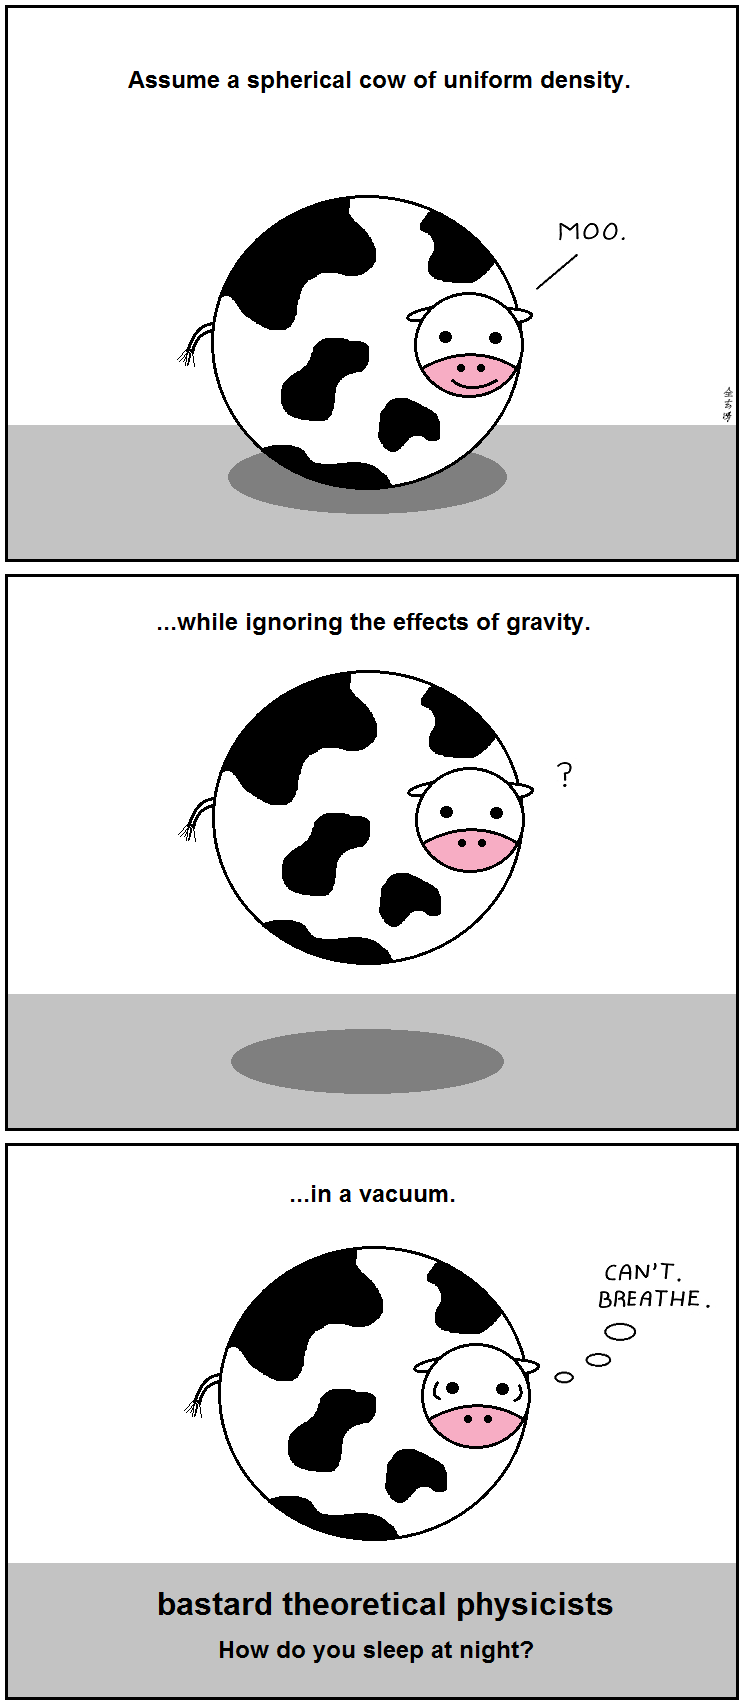
\includegraphics[trim={0 30cm 0 0},clip]{figures/spherical-cow.png}}
\end{center}

% http://abstrusegoose.com/406

\begin{flushright}
{\small \url{http://abstrusegoose.com/406}}
\end{flushright}

\vfill
\end{slide}
 
%------------------------------------------------------------------------------

% circular velocity, Oort's constants


%------------------------------------------------------------------------------
\begin{slide}
\begin{center}
{\large \color{red} 
                      Spherical Systems -- Important Quantities}
\end{center}

The velocity of a test particle on a circular orbit is the {\bf circular speed}, $v_c$.  
Setting the centripetal acceleration equal to the force we get
%\eq{
%v_c^2 = r {\d \Phi \over \d r} = r |\b F| = {G M(r) \over r}.
%}
\eq{
\frac{m v_c^2}{r} = |\b F| = {\d \Phi \over \d r} = {G M(r) m \over r^2} \,\,\, \Rightarrow \,\,\, v_c = \sqrt{ G M(r) \over r}
}
The circular speed is a measure of the mass interior to $r$, $M(r)$.

If $v_c$ as a function of $r$ is known, and we {\it assume that the
potential is spherical}, we can compute the mass as a function of $r$
(not the case for a non-spherical distribution.)

\vfill
\end{slide}

%------------------------------------------------------------------------------
\begin{slide}
\begin{center}
{\large \color{red} 
                      Spherical Systems -- Important Quantities}
\end{center}

Another important quantity is the {\bf escape speed}, $v_e$, defined by
\eq{
v   _e(r) = \sqrt{2 | \Phi (r)|}.
}
This definition comes from setting the kinetic energy of a star equal
to the absolute value of its potential energy.  That is, stars with
positive total energy are not bound to the system.
In order for a star to escape from from the gravitational field
represented by $\Phi$, it is necessary that its speed be greater than
$v_e$.  This can be used to get the local $\Phi$ of the galaxy.

\vfill
\end{slide}


%------------------------------------------------------------------------------
\begin{slide}
\begin{center}
{\large \color{red} 
                      Spherical Systems -- Simple Examples}
\end{center}

{\bf Let's look at something we're familiar with -- a point mass:}
\eq{
\rho(r) = M \delta(r) \mspace \Rightarrow \mspace \Phi(r) = -{ G M \over r} \mspace 
}
Plugging it into equations from previous slides, we find:
\eq{
v_c(r) = \sqrt{G M \over r} \mspace ; \mspace v_e(r) = \sqrt{2 G M \over r}.
}
Whenever the circular speed declines as $r^{-1/2}$, it is referred to as
{\bf \color{red} Keplerian}.  It usually implies that there is no significant mass
at that radius.

\vfill
\end{slide}

%------------------------------------------------------------------------------
\begin{slide}
\begin{center}
{\large \color{red} 
                      Spherical Systems -- Simple Examples}
\end{center}

{\bf Homogeneous sphere:}
\eq{
M = \frac{4}{3} \pi r^3 \rho \mspace ; \mspace v_c = \sqrt{4 \pi G
\rho \over 3} r.
}
The equation of motion for a particle in such a body is
\eq{
{\d^2 r \over \d t^2} = - { G M(r) \over r^2} = - {4 \pi G \rho \over
3} r,
}
which describes a harmonic oscillator with period
\eq{
T = \sqrt{3 \pi \over G \rho}.
}

\vfill
\end{slide}


%------------------------------------------------------------------------------
\begin{slide}
\begin{center}
{\large \color{red} 
                      Spherical Systems -- Simple Examples}
\end{center}


Independent of $r$, if a particle is started at $r$, it will reach the
center in a time
\eq{
t_{dyn} = {T \over 4} = \sqrt{ 3 \pi \over 16 G \rho},
}
known as the {\bf dynamical time}.  Although this result is only true
for a homogeneous sphere, it is a common practice to use this definition
with any system of density $\rho$.

By integrating the density for a homogeneous sphere, we can get the potental:
$$
\Phi = \left\{ \begin{array}{ll} -2\pi G \rho(a^2 - \frac{1}{3} r^2),
& r < a \\ - {4\pi G \rho a^3 \over 3 r}, & r > a. \end{array}\right.
$$

One would expect the center of a galaxy to have a potential of this
type if there is no cusp in the central density (implying a linear
rise in $v_c$).



\vfill
\end{slide}



%------------------------------------------------------------------------------
\begin{slide}
\begin{center}
{\large \color{red} 
                      Spherical Systems -- Simple Examples}
\end{center}


{\bf Isochrone potential:}
\eq{
\Phi(r) = - {GM \over b + \sqrt{b^2 + r^2}}.
}
This has the nice property of going from a harmonic oscillator in the
middle to a Keplerian potential at large $r$, with the transition
occurring at a scale $b$.

The circular speed is
\eq{
v_c^2 = {GMr^2 \over (b + a)^2 a},
}
where $a \equiv \sqrt{b^2 + r^2}$.

\vfill
\end{slide}


%------------------------------------------------------------------------------
\begin{slide}
\begin{center}
{\large \color{red} 
                      Spherical Systems -- Simple Examples}
\end{center}


Using Poisson's equation ($\nabla^2 \Phi = 4\pi G \rho$), we can find the density:

\eq{
\rho(r) = {1 \over 4\pi G r^2} {\d \over \d r}\left(r^2{\d \Phi \over
\d r}\right) = M \left[{3(b+a)a^2 - r^2(b + 3a) \over 4\pi(b+a)^3a^3}\right].
}

So the central density is
\eq{
\rho(0) = { 3 M \over 16 \pi b^3},
}
and the asymptotic density is
\eq{
\rho(r) \approx { b M \over 2\pi r^4}.
}

%Other commonly discussed profiles are 
%   {\bf modified Hubble profile} and {\bf power-law profile}.
\vfill
\end{slide}






%------------------------------------------------------------------------------
\begin{slide}
\begin{center}
{\large \color{red} 
                         Potential--Density Pairs }
\end{center}
The isochrone potential and density shown in previous slide was an example of
a {\bf potential-density pair}. These are equilibrium solution to Newtonian 
equations of motion that are similar to observed density and kinematic
profiles.

Other frequently used models include:

{\bf Plummer's (1911) model:} spherically symmetric, originally used to model globular clusters \\
{\bf Kuzmin's (1956) model:} infinitely thin disk (aka {\it Toomre's model 1}) \\
{\bf Plummer--Kuzmin models':} introduced by Miyamoto \& Nagai (1975), smooth transition from Plummer's to Kuzmin's models \\
{\bf Logarithmic potentials:} the circular speed is a constant at large radii
(very frequently used because of this property).

\vfill
\end{slide}





%------------------------------------------------------------------------------

\begin{slide}
\begin{center}
{\large \color{red} 
                 The Milky Way Density and Potential      }
\end{center}

The most popular Milky Way {\em stellar density} models are double exponential disk (thin and 
thick in the $Z$ direction, also exponential dependence in the $R$ 
direction), with a power-law or logarithmic halo.

But when kinematic information is taken into account, we discover that these
distributions would not be in dynamic equilibrium all by themselves.  This
leads us to postulate the existence of an additional, dark, matter component
(more in Lecture 10).

{\color{blue} Some recent good reviews:}

Bahcall (1986, ARA\&A 24, 577)

Gilmore, Wyse \& Kuijken (1989, ARA\&A 27, 555)

Majewski (1993, ARA\&A 31, 575)

Freeman \& Bland-Hawthorn (2002, ARA\&A 40, 487)


\vfill
\end{slide}





%------------------------------------------------------------------------------

\begin{slide}
\begin{center}
{\large \color{red} 
                      Orbits in Static Spherical Potentials    }
\end{center}

{\color{blue} The problem: given the initial conditions
$\b x(t_o)$ and $\dot \b x(t_o)$, and the potential $\Phi(r)$, find
$\b x(t)$.}

{\bf Orbits in spherical potentials are easy to consider and lead to some
important concepts.}


\begin{itemize}
\item Some general considerations
\item Example 1: Spherical harmonic oscillator: $\Phi(r) = A + B\,r^2$
\item Example 2: Point mass potential: $\Phi(r) = {-GM \over r}$
\item Example 3: Isochrone potential: $\Phi(r) = {-GM \over b + \sqrt{b^2 + r^2}}$
\end{itemize}

\vfill
\end{slide}



%------------------------------------------------------------------------------

\begin{slide}
\begin{center}
{\large \color{red} 
                   General considerations   }
\end{center}

{\color{blue} The initial conditions are 6-dimensional and thus a general solution
includes six orbital parameters.} (aka {\it constants of motion})

The equation of motion in a spherical potential is:
\eq{
\ddot \b r = F(r) \hat \b e_r,
}
i.e. the force is always (unsurprisingly) radial.

Crossing through by $\b r$, we show that the angular momentum vector,
$\b L \equiv \b r \times \dot \b r$ is conserved:
\eq{
  \ddt{} \left( \b r \times \dot \b r \right) = 
\ddt{\b r} \times \ddt{\b r} + \b r \times \ddtS{\b r} = {\b r} \times F(r) \hat \b e_r = 0
}

Therefore, the motion is constrained to the plane perpendicular to $\b L$,
and can be fully described in cylindrical coordinate system, $r$ and $\psi$
($\b v = \dot r \, \hat \b e_r + r \dot \psi \, \hat \b e_{\psi}$)

\vfill
\end{slide}



%------------------------------------------------------------------------------
\begin{slide}
\begin{center}
{\large \color{red} 
                   General considerations   }
\end{center}

The equations of motion in the plane are
\begin{eqnarray*}
\color{blue} \ddot r - r\dot\psi^2 & \color{blue} = & \color{blue} F(r) \\
\color{blue} 2 \dot r \dot \psi + r \ddot \psi & \color{blue} = & \color{blue} 0.
\end{eqnarray*}
The second equation comes from $r^2 \dot \psi = L =$ const. (note that this
is the second Kepler's law!)

$\dot \psi$ can be eliminated using $\dot \psi = L / r^2$, leading
to a one-dimensional equation of motion:
\eq{
\ddot r - L^2 / r^3 = F(r).
}

This equation motivates a definition of an effective potential
\eq{
- \nabla \Phi_{\rm eff} \equiv F(r) + L^2 / r^3,
}
and thus
\eq{
\Phi_{\rm eff}(r) \equiv \Phi(r) + {L^2 \over 2 r^2}.
}

\vfill
\end{slide}



%------------------------------------------------------------------------------
\begin{slide}
\begin{center}
{\large \color{red} 
                   General considerations   }
\end{center}

The energy per unit mass is
\eq{
     E = {1 \over 2} v^2 + \Phi(r) = {1 \over 2} (\dot r^2 + r^2 \dot \psi^2) + \Phi(r) = 
         {1 \over 2} \left( \dot r^2 + \Phi_{\rm eff}(r) \right).
}

We can transform this expression into $\dot r = dr/dt = f(E, L, r)$, and
integrate over $r$ fg
to find the period. For bound orbits $r$ oscillates between an inner radius, or {\color{red} pericenter}
($r_{\rm min}$), and an outer radius, or {\color{red} apocenter} ($r_{\rm max}$). The
{\bf radial period} is \eq{
  T_r = 2 \int_{r_{\rm min}}^{r_{\rm max}} (\sqrt{2[E-\Phi_{\rm eff}(r)]})^{-1}\, dr
}

The pericenter and apocenter are the solutions of $\Phi_{\rm eff}(r) = E$.

\vfill
\end{slide}



%------------------------------------------------------------------------------
\begin{slide}
\begin{center}
{\large \color{red} 
                   General considerations   }
\end{center}

The {\bf azimuthal period} is 
\eq{
            T_\psi = {2\pi \over \Delta \psi} T_r
}
where
\eq{
\Delta \psi = 2 L\, \int_{r_{\rm min}}^{r_{\rm max}} (r^2\,\sqrt{2[E-\Phi_{\rm eff}(r)]})^{-1}\, dr
}

{\bf The orbit is closed only for $\Delta \psi = k (2\pi)$ -- in general case,
the orbit forms a rosette.}

{\color{red} The orbital precession rate:}
\eq{
              \Omega_p = {\Delta \psi - 2\pi \over T_r}
}

\vfill
\end{slide}



%------------------------------------------------------------------------------
\begin{slide}
\begin{center}
{\large \color{red} 
                   General considerations   }
\end{center}

If we eliminate $t$ rather than $\psi$, then we have an equation for
the orbit's shape.  In terms of the variable {\color{red} $u \equiv 1/r$}
\eq{
{\d^2 u \over \d \psi^2 } + u = -{ F(u) \over L^2 u^2} \,\,\,\,\,
\Rightarrow \,\,\,\,\ {\d^2 u \over \d \psi^2 } = \zeta(u).
}

This is a second order differential equation for $u(\psi)$, where $\zeta(u)$
and the initial conditions are presumably specified.  It is not analytically
soluble in the general case, but analytic solutions exist for a few commonly
encountered potentials.

Let's now look at specific examples.
\vfill
\end{slide}




%------------------------------------------------------------------------------
\begin{slide}
\begin{center}
{\large \color{red} 
                         The harmonic potential    }
\end{center}

\eq{
\Phi = \Phi_0 + \frac{1}{2} \Omega^2 r^2.
}
Generated by homogeneous density distribution.

The motion decouples in cartesian co-ordinates to $\ddot x = -\Omega^2 x$ 
and $\ddot y = -\Omega y$, and the solution is:
\eq{
    x = X \cos(\Omega t + \phi_x), \mspace y = Y \sin(\Omega t + \phi_y),
}
where $X$, $Y$, $\phi_x$ and $\phi_y$ are arbitrary constants (determined
from initial conditions). 

This is the equation for an ellipse {\bf centered} on the origin. 

Orbits are closed
since the periods for $x$ and $y$ oscillations are identical.



\vfill
\end{slide}




%------------------------------------------------------------------------------
\begin{slide}
\begin{center}
{\large \color{red} 
                Point mass (Keplerian) potential}
\end{center}

\eq{
\Phi(r) = {-GM \over r}
}
\eq{
{\d^2 u \over \d \psi^2 } + u = {GM \over L^2} \mspace \Rightarrow \mspace
u = {GM \over L^2} [ 1 + e \cos(\psi - \psi_0)].
}
This is the equation for an ellipse with one {\bf focus at the origin} and
eccentricity $e$ (the first Kepler's law).  The semi-major axis is 
$a = L^2/GM(1-e^2)$. 

The motion is periodic in $\psi$ with period $2\pi$.  
This gives a closed orbit with 
\eq{
         T_r = T_\psi = 2\pi\sqrt{a^3 \over GM} = 2\pi GM (2|E|)^{-3/2}
} 
Note that $T^2 \propto a^3$ -- the third Kepler's law!


\vfill
\end{slide}




%------------------------------------------------------------------------------
\begin{slide}
\begin{center}
{\large \color{red} 
                 Isochrone Potential }
\end{center}

\eq{
      \Phi(r) = {-GM \over b + \sqrt{b^2 + r^2}}
}
More extended than point mass, less extended than harmonic potential.

$T_r$ same as for the Keplerian case ($T_r = 2\pi GM (2|E|)^{-3/2}$).

However, 
\eq{
       \Delta \psi = \pi \left[ 1 + {L \over \sqrt{L^2 + 4GMb}} \right]
}
i.e. $\pi < \Delta \psi < 2 \pi$, and hence {\bf the orbits are not closed!}



\vfill
\end{slide}

%------------------------------------------------------------------------------
\begin{slide}
\begin{center}
{\large \color{red} 
                       Axisymmetric Potentials   }
\end{center}

{\color{blue} The problem: given the initial conditions
$\b x(t_o)$ and $\dot \b x(t_o)$, and the potential $\Phi(R,z)$, find
$\b x(t)$.}

{\bf A better description of real galaxies than spherical potentials, 
and the orbital structure is much more interesting.}


\begin{itemize}
\item Poisson's equation for axisymmetric potentials, meridional plane
%\item Examples: $\Phi(x,y) = A\,x^2 + B\,y^2$} (non-axisymmetric)
%\item Example 2: $\Phi(x,y) \propto ln(x^2 + y^2/q^2)$ (non-axisymmetric)
\item Non-axisymmetric examples
\item Epicycle approximation

\end{itemize}

\vfill
\end{slide}


%------------------------------------------------------------------------------
\begin{slide}
\begin{center}
{\large \color{red} 
                       Axisymmetric Potentials   }
\end{center}

The equations of motion in an axisymmetric potential (cylindrical
coordinates) are
\eq{
     \ddot R = -{\p \Phi_{\rm eff} \over \p R} 
}
and
\eq{\ddot z = -{\p \Phi_{\rm eff} \over \p z}
}
where
\eq{
    \Phi_{\rm eff} \equiv \Phi + {L_z^2\over 2 R^2}
}
The total angular momentum is not conserved any more (we've broken the
rotational symmetry!), but its $\hat z$ component is:
\eq{
{\d \over \d t}(R^2 \dot\phi) = 0 \mspace \Rightarrow \mspace R^2
\dot\phi = L_z.
}


\vfill
\end{slide}



%------------------------------------------------------------------------------
\begin{slide}
\begin{center}
{\large \color{red} 
                       Axisymmetric Potentials   }
\end{center}

Hence, if we solve the first two equations, the solution for $\phi$
can be obtained from the last equation as

\eq{
    \phi(t) = \phi(t_o) + \dot \phi(t_o)\,R^2(t_o) \, \int_{t_o}^t dt'/R^2(t')
}

The three-dimensional motion in the cylindrical ($R,z,\phi$) space is
reduced to a two-dimensional problem in {\bf Cartesian} coordinates $R$ and
$z$.  Therefore, it's sufficient to study the motion of the particle in the
{\bf meridional plane} defined by $(R, z)$ coordinates.

\end{slide}

%------------------------------------------------------------------------------
\begin{slide}

\begin{center}
\vskip -0.0in
\scalebox{0.8}{\hskip 0.0in 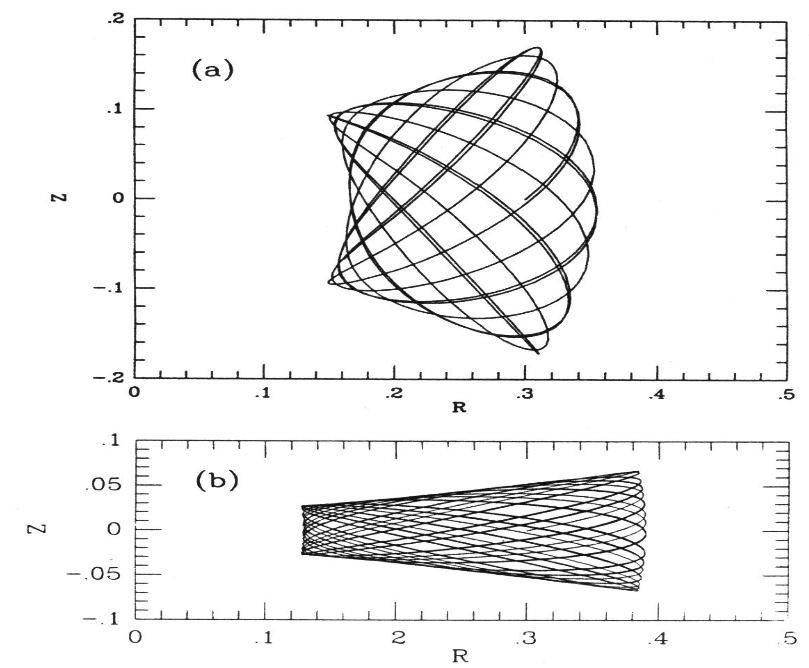
\includegraphics{figures/ex1.jpg}}
\end{center}


\vfill
\end{slide}


%------------------------------------------------------------------------------
\begin{slide}
\begin{center}
{\large \color{red} 
                       Axisymmetric Logarithmic Potential   }
\end{center}

A good approximative model to illustrate the properties of orbits in
axisymmetric potentials is one of the form:

\eq{
   \Phi = \frac{1}{2} v_0^2 \ln \left( R^2 + { z^2 \over q^2} \right)
}

(e.g., see Binney \& Tremaine, figs. 3-2, 3-3 and 3-4). This potential
asymptotes to a 2D harmonic oscillator (a homogeneous sphere) close to the
center, and for $q = 1$ it is equivalent to the spherical logarithmic
potential which yields constant rotation curves.

What kinds of orbits do we find in this potential?

\vfill
\end{slide}


%------------------------------------------------------------------------------
\begin{slide}
\begin{center}
{\large \color{red} 
                       Loop Orbit  }
\end{center}

\begin{center}
\vskip 0.0in
\scalebox{1.1}{\hskip 0.0in 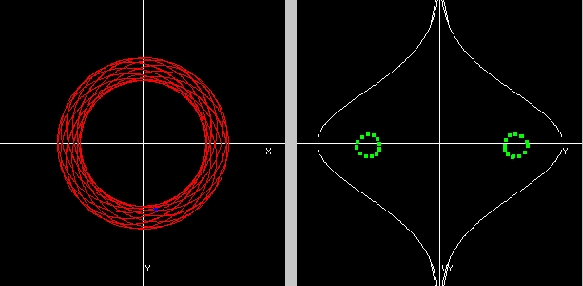
\includegraphics{figures/sos1.jpg}}
\end{center}

As mentioned earlier, the radial and azimuthal frequencies of an orbit
depend on the potential and generally aren't commensurate. In general, the
trajectory of a particle forms a {\em rosette}. If the particle moves so
that there's a sense of net rotation, the orbit is called a {\em loop} orbit.
(Above: a member of the 1:1 resonance family; more later).

\vfill
\end{slide}

%------------------------------------------------------------------------------
\begin{slide}
\begin{center}
{\large \color{red} 
                       Box Orbit }
\end{center}

\begin{center}
\vskip 0.0in
\scalebox{1.1}{\hskip 0.0in 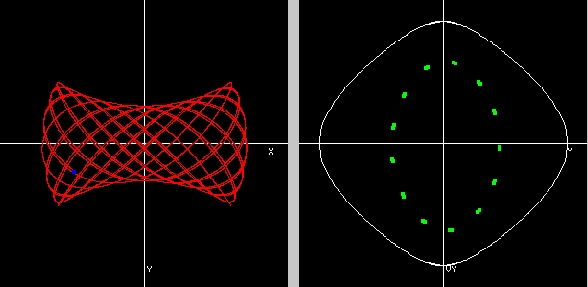
\includegraphics{figures/sos2.jpg}}
\end{center}

Orbits with no net sense of rotation belong to a class of {\em box orbits}. 
Particles in these orbits can get arbitrarily close to the center; over
time, they will completely fill the ``box'' in the $x-y$ plot.  A large
fraction of stars in {\bf galactic bars} are on box orbits (e.g.  Valluri
2016).

\vfill
\end{slide}

%------------------------------------------------------------------------------
\begin{slide}
\begin{center}
{\large \color{red} 
                       Banana Orbit }
\end{center}

\begin{center}
\vskip 0.0in
\scalebox{1.1}{\hskip 0.0in 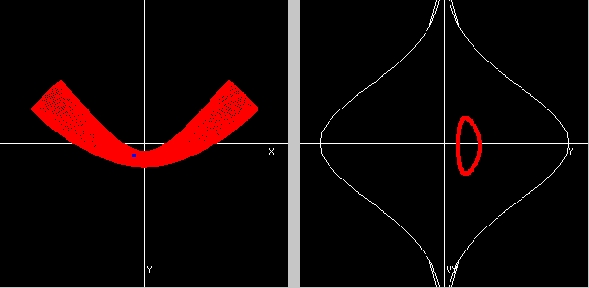
\includegraphics{figures/sos3.jpg}}
\end{center}

If oscillation frequencies are nearly commensurate we find orbits that are
more isolated in $x-y$ space. Above: a member of the ``bannana orbit''
family (associated with the 2:1 resonance).

\vfill
\end{slide}

%------------------------------------------------------------------------------
\begin{slide}
\begin{center}
{\large \color{red} 
                       X-shaped Bulge of the Milky Way }
\end{center}

\begin{center}
\vskip 0.0in
\scalebox{0.5}{\hskip 0.0in 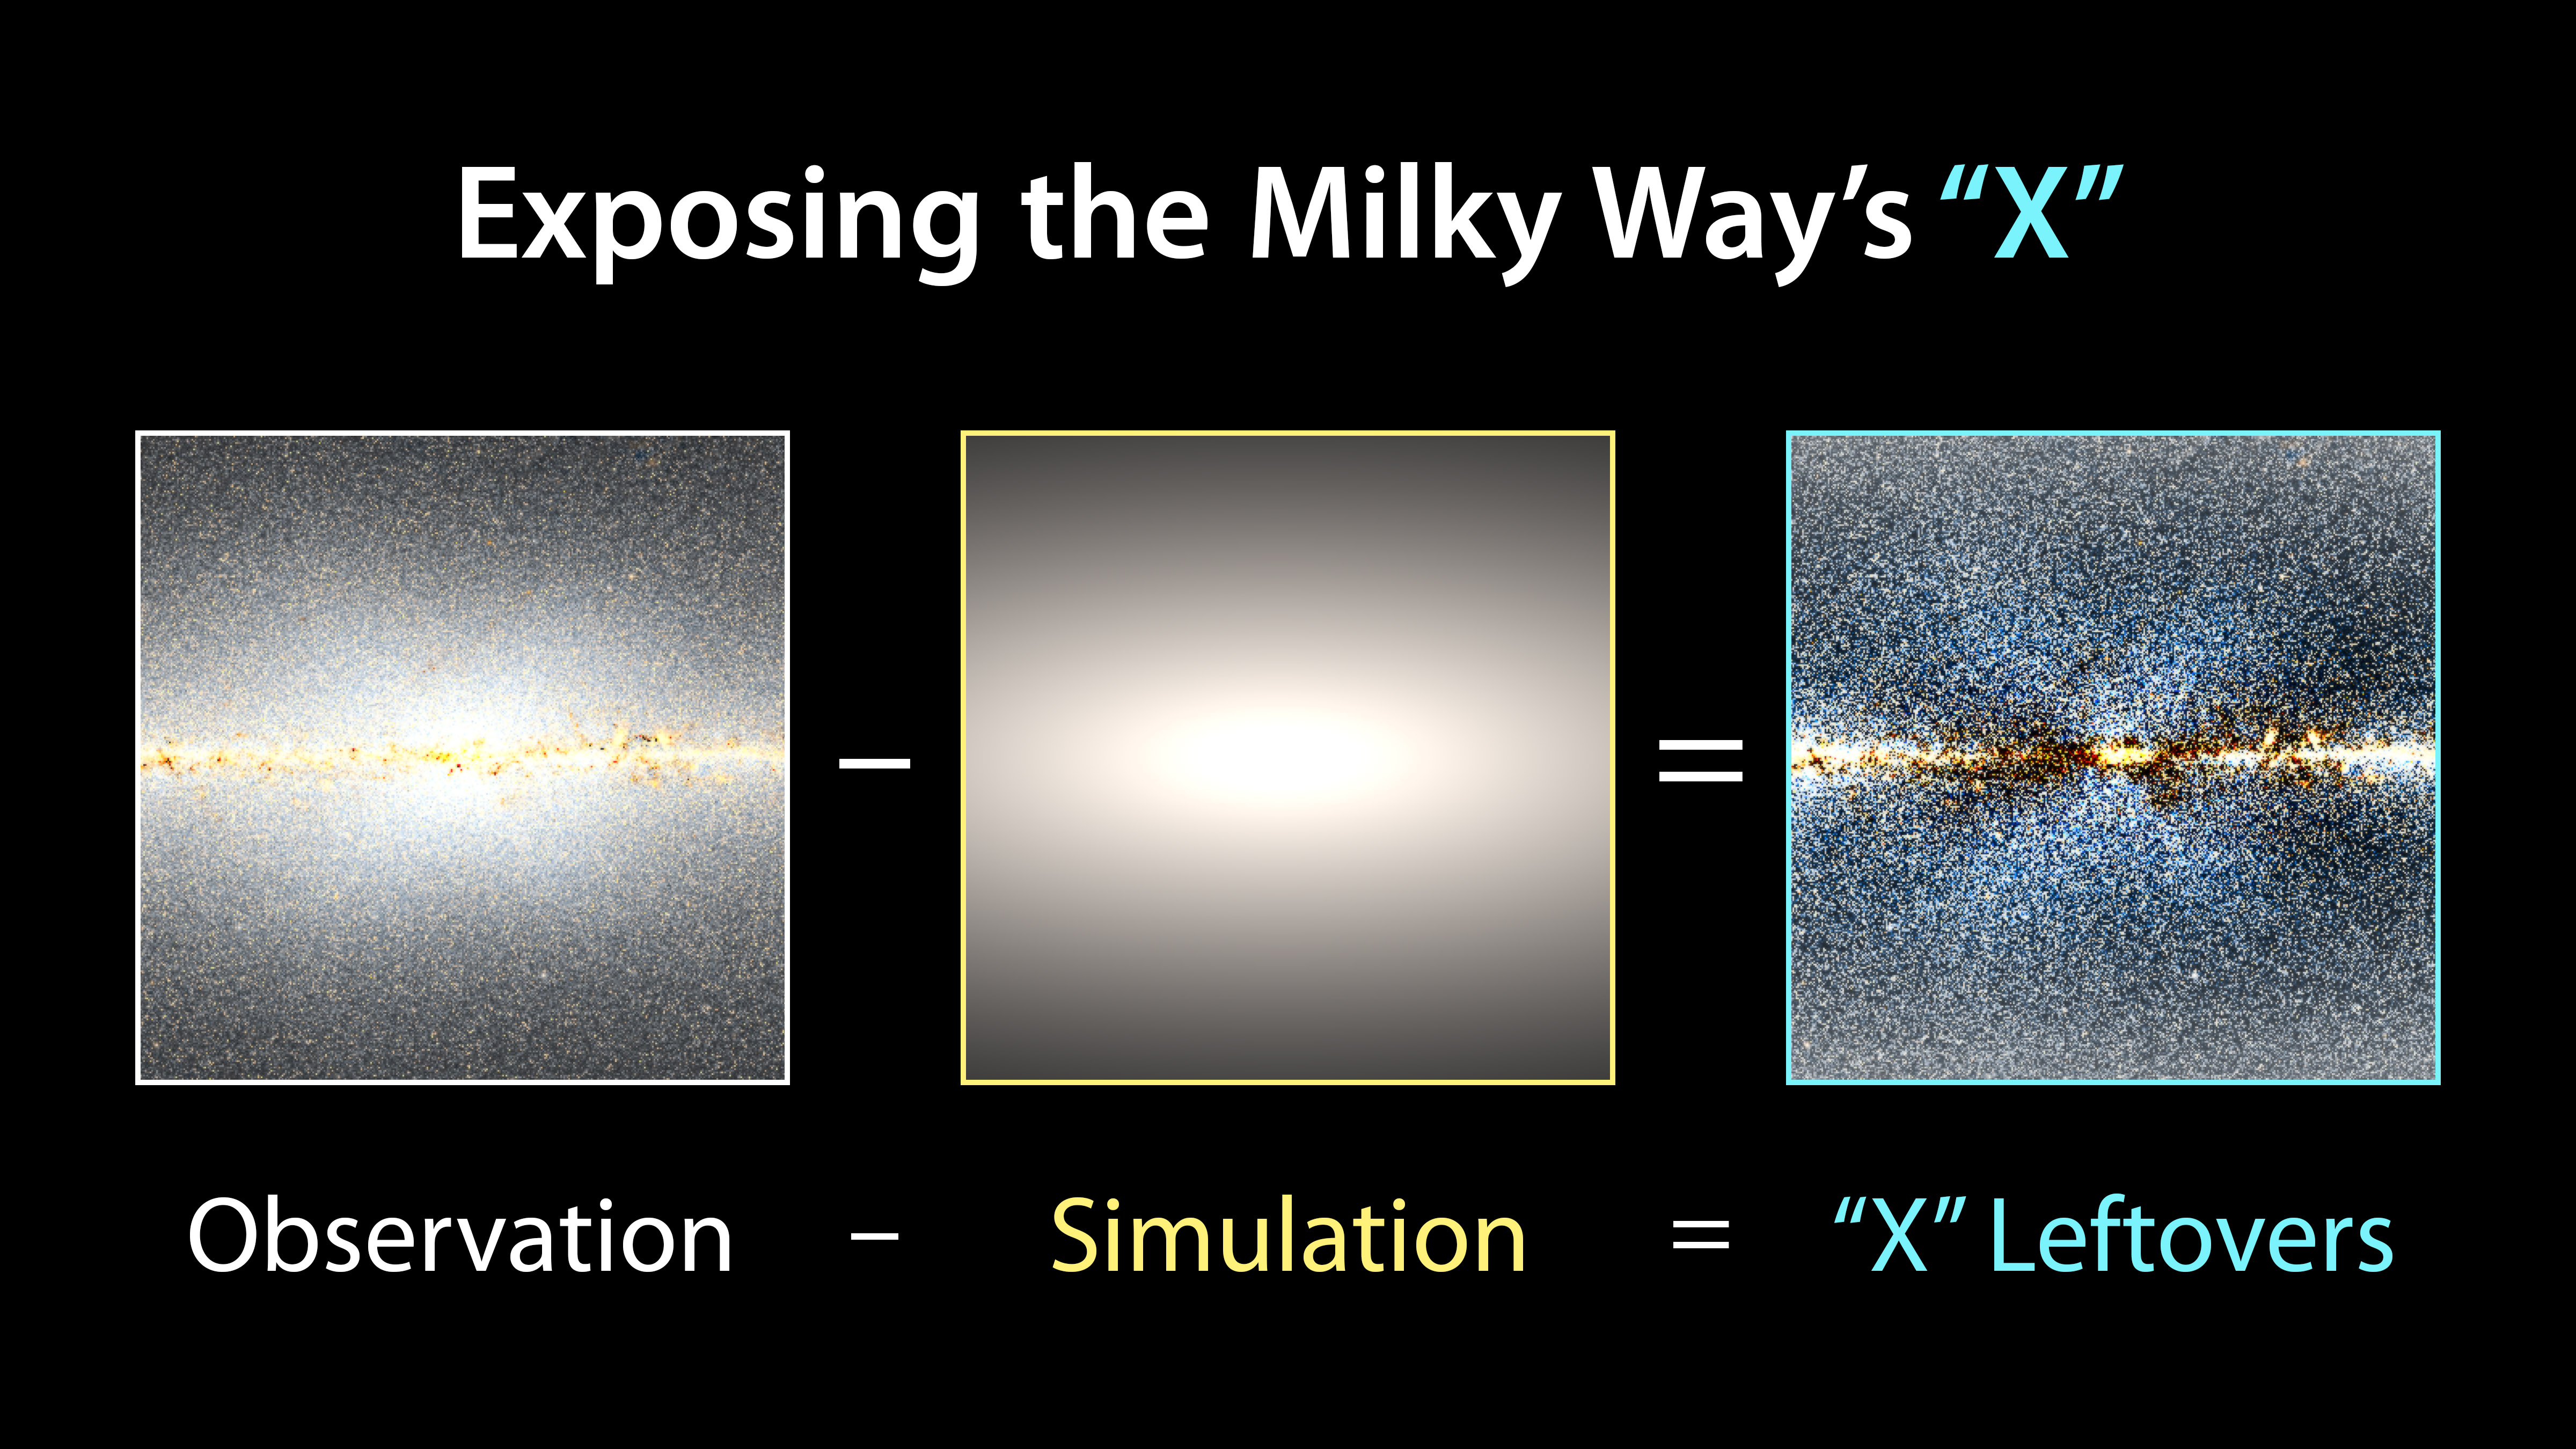
\includegraphics{figures/X3panel.jpg}}
\end{center}

X-shaped Bulge of the Milky Way as revealed by WISE (Ness \& Lang 2006;
\url{https://arxiv.org/pdf/1603.00026.pdf})

\vfill
\end{slide}

%------------------------------------------------------------------------------
\begin{slide}
\begin{center}
{\large \color{red} 
                      Fish Orbit  }
\end{center}

\begin{center}
\vskip 0.0in
\scalebox{1.1}{\hskip 0.0in 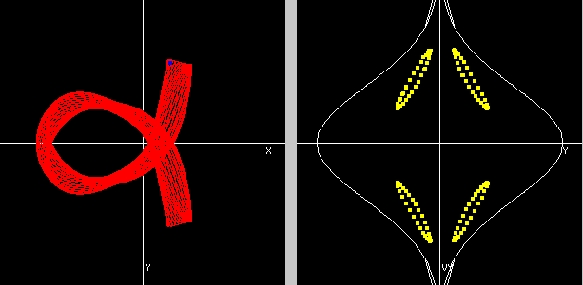
\includegraphics{figures/sos4.jpg}}
\end{center}

Above: a member of the ``fish orbit'' family (associated with the 3:2
resonance).

\vfill
\end{slide}

%------------------------------------------------------------------------------
\begin{slide}
\begin{center}
{\large \color{red} 
                    Box Orbit Scattered by a Point Mass  }
\end{center}

\begin{center}
\vskip 0.0in
\scalebox{1.1}{\hskip 0.0in 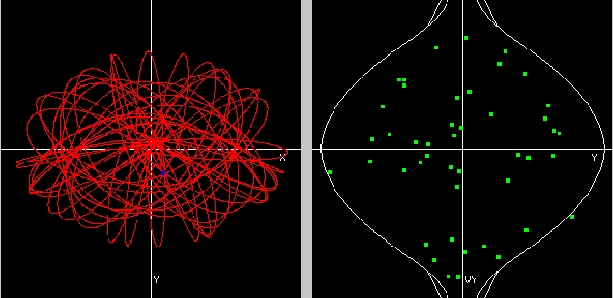
\includegraphics{figures/sos5.jpg}}
\end{center}

Adding a point mass into the center (e.g., a black hole), destroys the
order: a particle can get arbitrarily close to the center
and be scattered by the BH to a different orbit every time it does.
An extreme example: hypervelocity stars (Brown et al. 2005)

\vfill
\end{slide}








%------------------------------------------------------------------------------

\begin{slide}
\begin{center}
{\large \color{red} 
                       Axisymmetric Potentials: Insight into galaxy shapes   }
\end{center}

Studies of orbits in axisymmetric potentials give us insight into the origin
of structures observed in galaxies (rings, bulges, bars, etc.). This is a
rich area of theory to explore!

For an interesting recent article on how all this applies to the structure
of the Galactic bulge, see Portail, Wegg and Gerhard (2015; arXiv:1503.07203).

For a modern approach, see Thomas et al. 2004, MNRAS 353, 391: orbit
libraries, a Voronoi tessellation of the surface of section, the reconstruction
of phase-space distribution function

For a more classic orbital analysis (and if you are interested in finding
out what is an ``antipretzel''), see Miralda-Escud\'{e} \& Schwarzschild
1989 (ApJ 339, 752): Another classic paper is de Zeeuw 1985 (MNRAS 216, 272)
(interested in ``unstable butterflies''?)

\vfill
\end{slide}


%------------------------------------------------------------------------------
%
% Orbit structure of the logarithmic potential
%
%\begin{slide}
%
%\begin{center}
%\vskip 0.0in
%\scalebox{1.1}{\hskip 0.0in 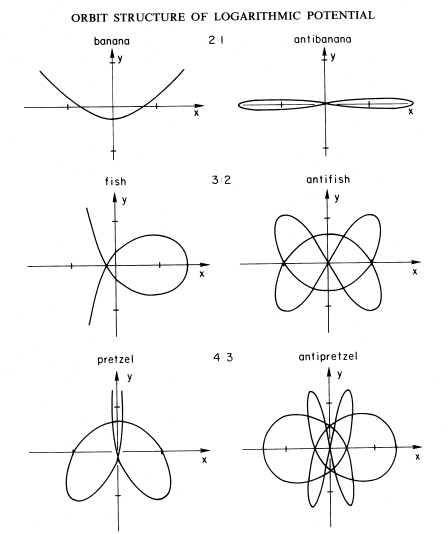
\includegraphics{figures/sos7.jpg}}
%\end{center}
%\vfill
%\end{slide}


%------------------------------------------------------------------------------
%
% Surfaces of section for orbits in logarithmic potentials
%
%\begin{slide}
%
%\begin{center}
%\vskip 0.0in
%\scalebox{1.1}{\hskip 0.0in 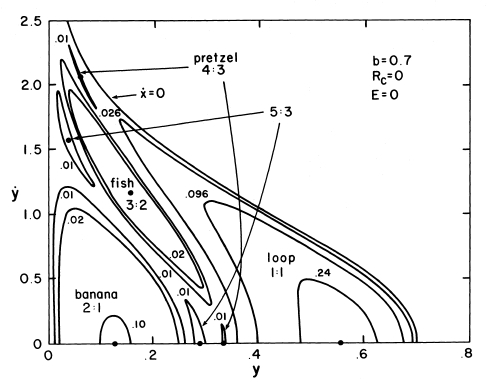
\includegraphics{figures/sos6.jpg}}
%\end{center}
%\vfill
%\end{slide}



%------------------------------------------------------------------------------

\begin{slide}
\begin{center}
{\large \color{red} 
                      Epicycle Approximation for Orbits  }
\end{center}

Assume an axisymmetric potential $\Phi_{\rm eff}$ and {\bf nearly
circular orbits};
expand $\Phi_{\rm eff}$ in a Taylor series about its minimum:
\eq{
\Phi_{\rm eff} = {\rm const} + \frac{1}{2} \kappa^2 x^2 + \frac{1}{2}
\nu^2 z^2 + \cdots,
}
where
\eq{
x \equiv R - R_g, \mspace \kappa^2 \equiv \left.{\p^2 \Phi_{\rm eff} \over
\p R^2}\right|_{(R_g, 0)}, \mspace \nu^2 \equiv \left.{\p^2 \Phi_{\rm
eff} \over \p z^2}\right|_{(R_g, 0)}.
}

The equations of motion decouple and we have two integrals:
\begin{eqnarray*}
x = X \cos(\kappa t + \phi_0) & \mspace & z = Z \cos(\nu t + \zeta) \\
E_R \equiv \frac{1}{2}[v_R^2 + \kappa^2(R - R_g)^2] & \mspace & E_z
\equiv \frac{1}{2}[v_z^2 + \nu^2 z^2].
\end{eqnarray*}

\vfill
\end{slide}


%------------------------------------------------------------------------------

\begin{slide}
\begin{center}
{\large \color{red} 
                      Epicycle Approximation   }
\end{center}


Now compare the {\bf epicycle frequency}, $\kappa$, with the angular
frequency, $\Omega$.
\eq{
\Omega^2 \equiv {v_c^2 \over R^2} = {1 \over R}{\p \Phi \over \p R} =
{1 \over R}{\p \Phi_{\rm eff} \over \p R} + {L_z^2 \over R^4},
}
\eq{
\kappa^2 = {\p(R^2 \Omega^2) \over \p R} + {3L_z^2 \over R^4} = R{\p
\Omega^2 \over \p R} + 4\Omega^2.
}

Since $\Omega$ always decreases, but rarely faster than Keplerian ($\Omega
\propto R^{-\frac{3}{2}}$):
\eq{
\Omega \le \kappa \le 2\Omega.
}

{\it These are not the infamous epicycles of Ptolemy's!} 
\vfill
\end{slide}


%------------------------------------------------------------------------------

\begin{slide}
\begin{center}
{\large \color{red} 
                      Epicycle Approximation   }
\end{center}

The epicycle approximation also makes a prediction for the
$\phi$-motion since $L_z = R^2 \dot\phi$ is conserved.  Let
\eq{
y \equiv R_g[\phi - (\phi_0 + \Omega t)]
}
be the displacement in the $\phi$ direction from the ``guiding
center''.  If we expand $L_z$ to first order in displacements from the
guiding center, we obtain
\eq{
\phi = \phi_0 + \Omega t - { 2 \Omega X \over \kappa R_g} \sin(\kappa
t + \phi_0).
}
Therefore
\eq{
y = -Y\sin(\kappa t + \phi_0) \hbox{\quad where\quad} {Y\over X} =
{2\Omega\over \kappa} \equiv \gamma \ge 1.
}
$\Rightarrow$ The epicycles are elongated tangentially (for Keplerian
motion $\gamma=2$: {\bf epicycles are not circles} as assumed by Hipparchus and 
Ptolomey!) 

\vfill
\end{slide}


%------------------------------------------------------------------------------

\begin{slide}

The epicycle frequency ($\kappa$) is related to {\bf Oort's constants}:
\eq{
   A \equiv {1 \over 2} \left( {v_c \over R} - {d v_c \over dR}\right)_{R_\odot}
 =  - {1 \over 2} \left( R {d\Omega \over dR}\right)_{R_\odot}
}
\eq{
   B \equiv - {1 \over 2} \left( {v_c \over R} + {d v_c \over dR}\right)_{R_\odot}
 = - \left( {1 \over 2} R {d\Omega \over dR} + \Omega \right)_{R_\odot}
 = A - \Omega_\odot
}
Then
\eq{
     \kappa_\odot^2 = -4B(A-B) = -4 B \Omega_\odot  
}
In the solar neighborhood,
\eq{
   A = 14.5\pm1.5 \,\, {\rm km/s/kpc}, \,\,\,\, B=-12 \pm 3 \,\, {\rm km/s/kpc},
}
and so
\eq{
    \kappa_\odot = 36 \pm 10 \,\, {\rm km/s/kpc},
}
and 
\eq{
       { \kappa_\odot \over  \Omega_\odot} = 1.3 \pm 0.2 \,\,\,\,  (>1 \, {\rm and} \, <2!)
}



{\color{red} For improvements to epicycle approximation see 
Dehnen 1999 (AJ 118, 1190)}

\vfill
\end{slide}



\end{document}


